
In general, the results of this project have been positive. A large number of images were generated and the environment was designed to make it quick and easy to produce even more images if needed. However, there are areas where improvements could enhance the datasets effectiveness for machine learning applications.

\section{Realism of the 3D Models and Environment}
The quality of the generated images was limited by the free assets used in the project. While the water simulation contributed to a sense of realism, other elements, such as docks and boats, relied on low-poly models. Low-poly models are simpler and less detailed than high-poly ones, which significantly impacted the overall realism of the scenes. \\

\noindent The lack of realism of the dataset can make it less suitable for computer vision tasks in real-world environments. For instance, sharp edges and simple object designs highlight the synthetic nature of the scenes, creating a domain gap between real-world scenes.

\subsection{Techniques to Bridge the Domain Gap}
Several techniques can be used to enhance the realism of synthetic data and bridge the domain gap, including:

\begin{itemize}
    \item \textbf{Synthetic-to-Real Refinement}: This approach uses domain adaptation models, such as Generative Adversarial Networks (GANs), to make synthetic data more visually realistic \cite{nikolenko2021synthetic}.

    \item \textbf{Model-based domain adaptation}: Here, the focus is on adapting the model or its training process rather than modifying the data itself. Different techniques are employed to enhance the model's ability to generalize across domains without changing the synthetic data \cite{nikolenko2021synthetic}.
\end{itemize}


\subsection{Combining AI with Unity for Enhancement}
A promising approach to improving synthetic environments is the use of AI-based tools to enhance realism. Tools like Stable Diffusion and DALL-E take an image and a text prompt as input, and will generate an altered image that reflects the given prompt. These models are highly effective at adding realistic details or modifying elements of an image to make it appear more natural \cite{aiToExoand}. \\

\noindent For example, Unity-generated images were enhanced using Stable Diffusion, accessed through the Dezgo platform \cite{Dezgo2024}. The AI adds photorealistic details, such as improving textures, adjusting lighting and subtly altering objects like boats or the background. These enhancements not only make the dataset more visually realistic but also introduce slight variations, increasing diversity and number of images in the dataset.\\

\noindent Figure \ref{fig:ai_promt} illustrates the input image and the text prompt was "Make it more photorealistic". Figure \ref{fig:ai_enhanced} demonstrates the results, showcasing the transformation of Unity-generated images after AI enhancement. This shows how the overall quality and realism of the dataset can improve, potentially making it more effective for real-world applications in machine learning.

\begin{figure}[H]
\centering
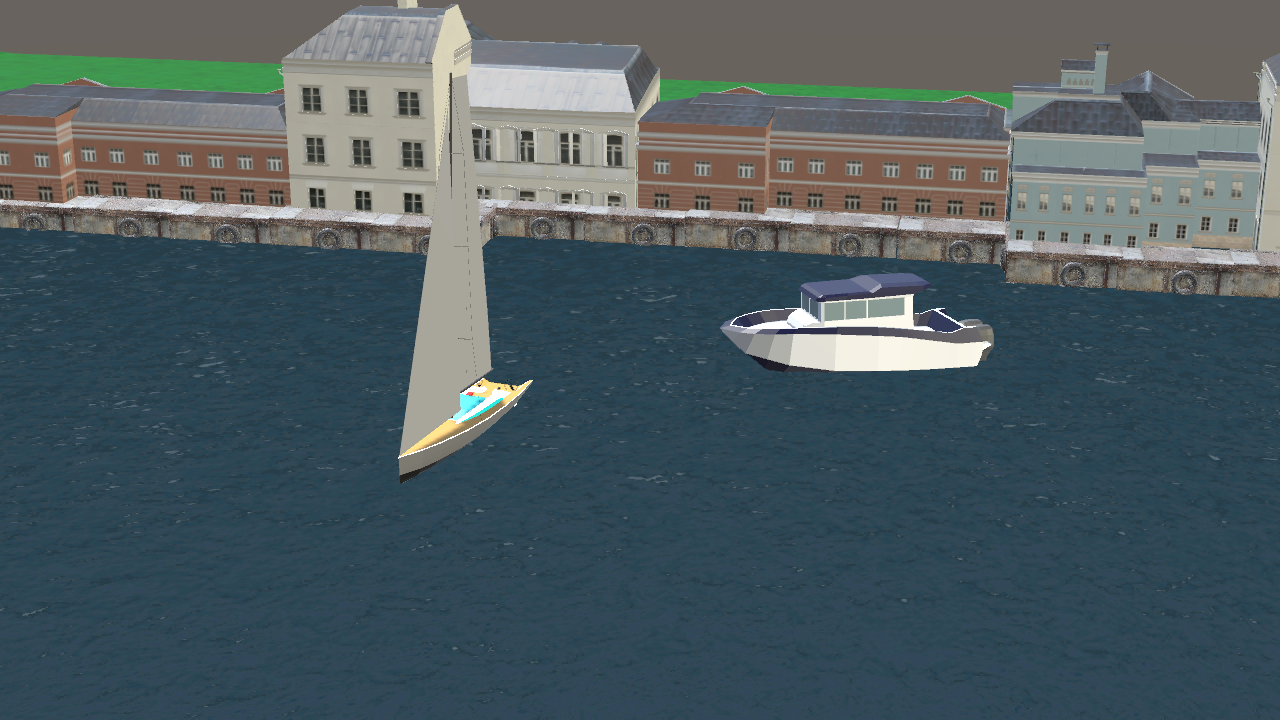
\includegraphics[width=0.6\textwidth]{Figures/rgb_2.png}
\caption{The initial image input to Dezgo platform.}
\label{fig:ai_promt}
\end{figure}

\begin{figure}[H]
\centering
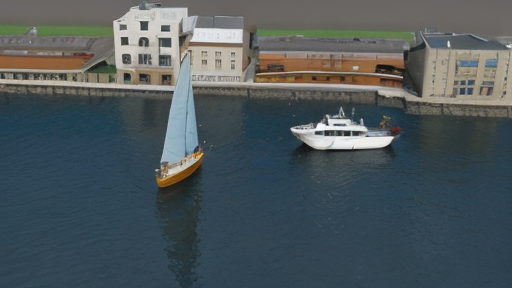
\includegraphics[width=0.49\textwidth]{Figures/results/photorealistic_3613113118.png}
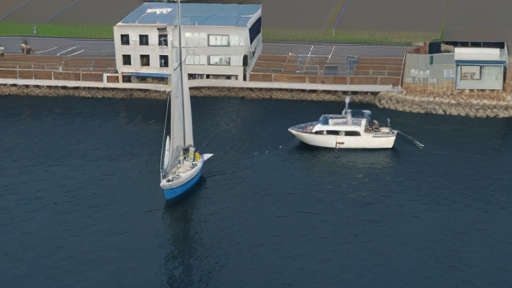
\includegraphics[width=0.49\textwidth]{Figures/results/photorealistic_2942539231.png}
\caption{AI-enhanced images generated using Dezgo platform.}
\label{fig:ai_enhanced}
\end{figure}

\noindent This method helps creating high-quality synthetic datasets with minimal additional effort, which is worth exploring further in the Master Thesis.


\section{Expanding the Dataset}
This setup allows for straightforward expansion of the dataset. With the environment already built and the Unity Perception Package \cite{unity-perception2022} integrated, additional images can be generated quickly and efficiently, ensuring the dataset can be scaled when required. \\

\noindent Another way to expand the dataset is by applying traditional augmentation techniques to the existing images. Techniques such as shifting, scaling, rotating, cropping and adding blur can introduce further variation without additional 3D rendering \cite{nikolenko2021synthetic}. These methods can enhance dataset diversity and improve the generalizability of machine learning models trained on it.


\section{Challenges and Limitations}
Several challenges arose during the project, particularly related to Unity version compatibility and asset rendering. For instance, imported materials were sometimes incompatible with the projects Unity version, causing objects to appear pink or fail to render altogether. These issues were especially challenging for water simulations, which limited the variety and realism of the scenes that could be created.\\

\noindent Additionally, the reliance on free or low-cost assets restricted the diversity and quality of objects available for use. This limitation not only reduced the range of scenarios represented in the dataset but also impacted the overall realism of the generated images.\\

\noindent To address these challenges, future projects could benefit from investing in higher-quality assets or collaborating with designers to develop custom 3D models tailored to specific needs. These improvements would enhance both the visual fidelity and the diversity of the dataset, making it more robust for training machine learning models.



